\documentclass[conference]{IEEEtran}
\IEEEoverridecommandlockouts

\usepackage{iftex}
\ifXeTeX
  \usepackage{fontspec}
  \setmainfont{texgyretermes}[Extension=.otf,UprightFont=*-regular,
    BoldFont=*-bold,ItalicFont=*-italic,BoldItalicFont=*-bolditalic]
\fi

\usepackage{cite}
\usepackage{amsmath,amssymb,amsfonts,amsthm}
\usepackage{graphicx}
\usepackage{booktabs}
\usepackage{multirow}
\usepackage{algorithm}
\usepackage{algorithmic}
\usepackage{listings}
\usepackage{xcolor}
\usepackage{url}
\def\UrlBreaks{\do\/\do-\do\_\do.}
\usepackage[hidelinks]{hyperref}

\newtheorem{proposition}{Proposition}
\newtheorem{remark}{Remark}
\DeclareMathOperator*{\argmax}{arg\,max}
\DeclareMathOperator{\softmax}{softmax}
\newcommand{\E}{\mathbb{E}}
\newcommand{\N}{\mathcal{N}}

\lstset{basicstyle=\ttfamily\scriptsize,columns=fullflexible,breaklines=true,
  frame=single,framerule=0.3pt,xleftmargin=2pt,xrightmargin=2pt}

\begin{document}

\title{Reverse-Engineering RLCD: What Reinforcement Learning Does (and Doesn't) Do for Calibrated Typed Decisions}

\author{\IEEEauthorblockN{Le Duc Minh}
\IEEEauthorblockA{Independent Researcher\\
Ho Chi Minh City, Vietnam\\
minh.leduc.0210@gmail.com}}

\maketitle

\begin{abstract}
``Reinforcement Learning for Calibrated Decisions'' (RLCD) is marketed as the
training method behind typed-decision models that return calibrated
probabilities over a closed set of options. The method behind the closed
model Jev is unpublished; the only open reproduction, Laya, trains with a
noisy-logit policy-gradient term added to soft cross-entropy (CE). We show
that this RL term is a score-function (evolution-strategies) estimator of
the gradient of a \emph{noise-smoothed} proper scoring rule. For the log
score, its optimum is provably sharper than the target at inference time,
with a gap that grows with the noise scale~$\sigma$. We then run a
13-configuration ablation that replicates Laya's fine-tune on the
typed-decisions benchmark. At fixed $\sigma\in\{0.5,1,2\}$, the fitted
temperature rises from 1.2 to 1.7 and target-referenced calibration error
rises from 0.054 to 0.111. At Laya's own annealed schedule, the RL term is
7--110$\times$ larger than the CE gradient, yet it changes nothing
measurable except a small loss in proper scores: CE-only is at least as
good on every metric we track. We also show that the benchmark's
hard-label ECE rewards over-sharpening, so it is unsuitable for this
question.
\end{abstract}

\begin{IEEEkeywords}
calibration, proper scoring rules, reinforcement learning, typed decisions,
non-autoregressive models, evolution strategies
\end{IEEEkeywords}

% =====================================================================
\section{Introduction}

A new class of ``System One'' models answers structured questions about
unstructured state in a single forward pass. Instead of generating text,
they return a probability distribution over a closed, typed set of options:
a \emph{choice} among named options, an ordinal \emph{score}, or a binary
\emph{noul} probability. TypeSafe's Jev~\cite{typesafe_blog} is the most
visible example. Its central promise is that the probabilities are
calibrated: an answer given with 0.8 confidence should be right about 80\%
of the time. The method credited for this, RLCD~\cite{rlcd_explained}, has
no published paper, reward function, dataset, or calibration
figure~\cite{typesafe_blog,techcrunch_jev}.

Laya~\cite{laya_repo} is an open, transparent attempt at the same
interface. It publishes code, checkpoints and an evaluation on the
\texttt{LocalLLaMA/typed-decisions} benchmark~\cite{typed_decisions_ds}.
Its training loop adds noise to the logits, rewards the noisy
distributions with a proper scoring rule, and applies a REINFORCE-style
update~\cite{williams1992reinforce} next to a soft CE term. Laya's own
README reports a raw ECE of 0.466 that drops to 0.081 after temperature
scaling. This suggests the RL objective, as implemented, does not by itself
produce calibration.

This report asks what that RL term actually does. Our contributions:
\begin{enumerate}
\item We show that Laya's RL term is an evolution-strategies
  estimator~\cite{salimans2017es,nesterov2017random} of the gradient of a
  noise-smoothed scoring rule, and that as $\sigma\to 0$ it recovers the CE
  gradient that is already present (Sec.~\ref{sec:analysis}).
\item We prove that for the log score and binary questions, the
  smoothed optimum is sharper than the target at noise-free inference, with
  a gap strictly increasing in~$\sigma$. We verify the same qualitative
  bias numerically for Laya's full reward and $K\le 77$ options
  (Sec.~\ref{sec:analysis}, \ref{sec:e1}).
\item We replicate Laya's fine-tune and ablate the loss in 13 runs
  (Sec.~\ref{sec:e2}). The predicted bias appears in full at fixed
  $\sigma\ge 0.5$. At Laya's annealed schedule the RL term dominates the
  update yet brings no benefit over CE-only.
\item We show that on this benchmark the gold labels are the teacher's
  argmax, so hard-label ECE \emph{improves} as models over-sharpen. We
  propose a target-referenced ECE that does measure the bias.
\end{enumerate}
Nothing in this report asserts how Jev is built. Statements about Jev are
restricted to TypeSafe's public claims and are labeled as inference.

% =====================================================================
\section{Background and Related Work}

\textbf{Calibration.} A predictor with confidence $c=\max_i p_i$ is
calibrated if $\Pr(\text{correct}\mid c)=c$. Expected calibration error
(ECE) estimates the gap with $B$ equal-width bins~\cite{naeini2015ece,guo2017calibration}:
\begin{equation}
\mathrm{ECE}=\sum_{b=1}^{B}\frac{|S_b|}{n}\,\Bigl|\,\overline{c}_{S_b}-\overline{a}_{S_b}\Bigr|,
\label{eq:ece}
\end{equation}
where $\overline{a}$ is the empirical accuracy in the bin; we use $B=15$ on
$c=\max_i p_i$. Temperature scaling~\cite{guo2017calibration} divides the
logits by a scalar $T$ fitted by NLL on held-out data. $T>1$ indicates
over-sharp raw outputs.

\textbf{Proper scoring rules.} A scoring rule $R(q,t)$ is strictly proper
if $\E_{y\sim t}R(q,y)$ is uniquely maximized at
$q=t$~\cite{gneiting2007scoring}. Laya combines three: the log score
$\sum_i t_i\log q_i$ (whose negative is soft CE), the spherical score
$\langle t,q\rangle/\|q\|$, and, for ordinal questions, the ranked
probability score (RPS)~\cite{epstein1969rps}. Brier~\cite{brier1950} is
$\|q-t\|_2^2$. Distillation onto teacher distributions~\cite{hinton2015distilling}
with soft CE already optimizes a strictly proper score.

\textbf{RLHF, RLVR, RLCD.} RLHF optimizes a learned preference
reward~\cite{christiano2017rlhf,ouyang2022instructgpt}. RLVR optimizes a
verifiable reward~\cite{lambert2024tulu3}, often with a group-mean baseline
as in GRPO~\cite{shao2024grpo}. RLCD, as publicly described, rewards
calibrated typed distributions~\cite{rlcd_explained}. Sampling a
distribution by perturbing logits and following the score function is
Gaussian smoothing, i.e.\ evolution strategies~\cite{salimans2017es,nesterov2017random,mohamed2020mcgrad}.

% =====================================================================
\section{Jev From the Outside (Inference)}
\label{sec:jev}

Table~\ref{tab:clues} maps TypeSafe's public claims~\cite{typesafe_blog,typesafe_docs,techcrunch_jev}
to design choices \emph{consistent with} them. Each row is an inference,
not a statement of fact. The claim relevant here is that no RL is needed to
optimize a proper score against distributions from a data engine one
controls: soft CE already does that exactly. RL earns its place only for
non-differentiable environment rewards, sequential decisions, or steering
data generation. None of these applies to Laya's training loop.

\begin{table}[t]
\caption{Public clues and designs consistent with them (inference only).}
\label{tab:clues}
\centering
\footnotesize
\begin{tabular}{@{}p{0.45\columnwidth}p{0.47\columnwidth}@{}}
\toprule
Public clue & Consistent design \\
\midrule
All answers in one query; output tokens ``free'' & prefill-only single forward pass \\
$\le$255 options per choice & closed option set, one logit per option \\
Negation pairs need not sum to 1 & independent per-question readouts \\
Weak arithmetic, dates, counting & single-pass ``System~1'' computation \\
Degrades with unrelated state & attention dilution over a long prefix \\
Trained only on synthetic data & a controlled data engine with known label distributions \\
\bottomrule
\end{tabular}
\end{table}

% =====================================================================
\section{Laya From the Inside}
\label{sec:laya}

\textbf{Model.} Each question is encoded as its own row:
\texttt{[CLS] <type> question: <instr> [SEP] [MASK] opt$_0$ [MASK] opt$_1$ \dots\ [SEP] <state> [SEP]}.
A ModernBERT-large encoder~\cite{warner2024modernbert} is followed by a
type embedding, two pre-norm transformer layers and an MLP scorer. The
scorer reads one logit $z_i$ at each option's \texttt{[MASK]} position,
and $p=\softmax(z/T)$ at inference. We ported this model and verified
tensor-for-tensor that Laya's released weights load into our port
(Appendix~\ref{app:repro}).

\textbf{Training step.} Algorithm~\ref{alg:laya} restates the training step
of Laya's typed-decisions fine-tune notebook~\cite{laya_repo}. Two details
differ from condensed descriptions of the method, and both matter. The
spherical weight is 0.75. The group-centered advantages are normalized by
\emph{their own} standard deviation; normalizing by the raw-reward standard
deviation instead shrinks the RL gradient $\sim$90$\times$ in our tests.

\begin{algorithm}[t]
\caption{Laya's RLCD training step (one batch).}
\label{alg:laya}
\begin{algorithmic}[1]
\REQUIRE rows with targets $t$, noise $\sigma$, samples $G{=}4$, weights $w_\mathrm{rl}{=}w_\mathrm{ce}{=}1$
\STATE $z \leftarrow f_\theta(x)$ \COMMENT{masked logits, $B\times K$}
\FOR{$g=1$ to $G$}
  \STATE $e_g\sim\N(0,\sigma^2 I)$;\ \ $\epsilon_g\leftarrow e_g-\bar e_g\mathbf{1}$ \COMMENT{zero mean over valid options}
  \STATE $q_g\leftarrow\softmax(\mathrm{sg}(z)+\epsilon_g)$;\ \ $r_g\leftarrow R(q_g,t)$
\ENDFOR
\STATE $a_g\leftarrow r_g-\tfrac1G\sum_{g'}r_{g'}$;\ \ $a\leftarrow a/(\mathrm{std}(a)+10^{-6})$
\STATE $L_\mathrm{RL}\leftarrow-\tfrac{1}{GB}\sum_g a_g\log\N(\mathrm{sg}(z)+\epsilon_g\mid z,\sigma^2 I)$
\STATE $L_\mathrm{CE}\leftarrow-\tfrac1B\sum t^\top\log\softmax(z)$
\STATE step on $w_\mathrm{rl}L_\mathrm{RL}+w_\mathrm{ce}L_\mathrm{CE}$ (clip 1.0, AdamW)
\end{algorithmic}
\end{algorithm}

Here $R(q,t)=\sum_i t_i\log q_i+0.75\,\langle t,q\rangle/\|q\|-\mathbb{1}[\text{score}]\,\mathrm{RPS}(q,t)$,
and $\mathrm{sg}$ denotes stop-gradient. $\sigma$ is annealed linearly
from 0.4 to 0.1 over four epochs. After training, one temperature per type
is fitted on a held-out slice (Laya issue \#186~\cite{laya_issue186}
records an earlier version that fitted it on training items).

% =====================================================================
\section{Analysis of the RL Term}
\label{sec:analysis}

\subsection{The RL term estimates a smoothed objective}

Let $P=I-\tfrac1K\mathbf{1}\mathbf{1}^\top$ and $\epsilon\sim\N(0,\sigma^2P)$,
the zero-mean-projected noise of Algorithm~\ref{alg:laya}. Define
\begin{equation}
J_\sigma(z)=\E_{\epsilon}\bigl[R(\softmax(z+\epsilon),t)\bigr].
\label{eq:jsigma}
\end{equation}
Since $\nabla_z\log\N(\mathrm{sg}(z)+\epsilon\mid z,\sigma^2 I)=\epsilon/\sigma^2$,
the gradient of $L_\mathrm{RL}$ is
\begin{equation}
-\nabla_z L_\mathrm{RL}=\frac{1}{GB\,\sigma^2}\sum_{g}a_g\,\epsilon_g,
\label{eq:es}
\end{equation}
a group-baselined Monte-Carlo estimate of the Gaussian-smoothing identity~\cite{nesterov2017random,mohamed2020mcgrad}
\begin{equation}
\begin{split}
\nabla_z J_\sigma(z)&=\tfrac{1}{\sigma^2}\,\E\bigl[R(\softmax(z+\epsilon),t)\,\epsilon\bigr]\\
&=P\,\E\bigl[\nabla_u R(\softmax(u),t)\big|_{u=z+\epsilon}\bigr],
\end{split}
\label{eq:stein}
\end{equation}
where the second equality is Stein's lemma. For the log score,
$\nabla_u R=t-\softmax(u)$, so as $\sigma\to0$ the RL term estimates
$t-\softmax(z)$, which is exactly the negative CE gradient. The RL term is
thus a noisy estimate of a gradient that the CE term already supplies
exactly, plus a $\sigma$-dependent deviation.

\subsection{The smoothed optimum is over-sharp}

For the log score, $J_\sigma$ is concave (an average of concave
log-softmax terms), so its maximizers are the stationary points
\begin{equation}
\E_\epsilon\bigl[\softmax(z^\star_\sigma+\epsilon)\bigr]=t .
\label{eq:stationary}
\end{equation}
The \emph{noise-averaged} prediction matches the target, but inference
reports the \emph{noise-free} $\softmax(z^\star_\sigma)$. For binary
questions (noul, $K{=}2$) the consequence can be proved exactly. With
projected noise, the logit gap $d=z_1-z_2$ receives
$\eta=\epsilon_1-\epsilon_2\sim\N(0,2\sigma^2)$, and \eqref{eq:stationary}
becomes $F_\sigma(d^\star):=\E[s(d^\star+\eta)]=t_1$ with $s$ the logistic
function.

\begin{proposition}
\label{prop:binary}
Let $K=2$, the log score, and $t_1\in(\tfrac12,1)$. For every $\sigma>0$
there is a unique maximizer $d^\star_\sigma$. It satisfies
$s(d^\star_\sigma)>t_1$, and $s(d^\star_\sigma)$ is strictly increasing in
$\sigma$ (symmetrically for $t_1<\tfrac12$).
\end{proposition}

\begin{proof}
Let $g=s-\tfrac12$. It is odd, increasing, and concave on $[0,\infty)$,
with $g''(x)=s(1-s)(1-2s)$ odd and negative for $x>0$. Fix $d>0$ and pair
$\pm\eta$. If $|\eta|\le d$, concavity gives
$g(d+\eta)+g(d-\eta)\le 2g(d)$. If $|\eta|>d$, then
$g(d+|\eta|)+g(d-|\eta|)=g(|\eta|+d)-g(|\eta|-d)$. This is the increment
of a concave function over an interval of length $2d$ starting at
$|\eta|-d>0$, so it is at most $g(2d)-g(0)\le 2g(d)$, strictly for
$\eta\neq0$. Hence $F_\sigma(d)<s(d)$ for all $d>0$. The map $F_\sigma$ is
continuous and strictly increasing, with $F_\sigma(0)=\tfrac12$ and
$F_\sigma(\infty)=1$, so $F_\sigma(d)=t_1$ has a unique root $d^\star>0$,
and $s(d^\star)>F_\sigma(d^\star)=t_1$. For monotonicity, write
$\eta=\tau Z$ with $\tau=\sqrt2\sigma$. By Stein's lemma,
$\partial_\tau\E[g(d+\tau Z)]=\tau\,\E[g''(d+\tau Z)]$. Because $g''$ is odd
and negative on $(0,\infty)$, and the Gaussian centered at $d>0$ puts more
mass at $+x$ than at $-x$, this expectation is negative. So $F_\sigma(d)$
decreases in $\sigma$ at fixed $d$. Keeping $F_\sigma(d^\star_\sigma)=t_1$
therefore requires $d^\star_\sigma$ to increase with $\sigma$, and $s$ is
increasing.
\end{proof}

\begin{remark}[size of the bias]
A second-order expansion gives
$\E[\softmax(z+\epsilon)]=\softmax(z)+\tfrac{\sigma^2}{2}\sum_{jk}P_{jk}\partial_j\partial_k\softmax(z)+O(\sigma^4)$.
The optimum therefore deviates from $t$ by $O(\sigma^2)$. Under Laya's
schedule ($\sigma\le0.4$, ending at 0.1) the deviation is 6--100$\times$
smaller than at $\sigma=1$. This predicts that Laya's recipe is nearly
unbiased but gains nothing over CE, which is what Sec.~\ref{sec:e2}
finds.
\end{remark}

For $K>2$ and for Laya's full reward we rely on numerics
(Sec.~\ref{sec:e1}). Temperature scaling can undo much of the
distortion: at the optimum, noise-free outputs are approximately the
target sharpened, and a uniform $T>1$ reverses most of that.

\subsection{Variance and advantage normalization}

After normalization the advantages are $O(1)$ regardless of the reward
scale, so \eqref{eq:es} has norm $\propto\|\epsilon\|/\sigma^2\propto
1/\sigma$. As $\sigma$ anneals, the RL term grows relative to CE. It is
estimated from only $G{=}4$ samples, and the batch-wide standard deviation
rescales the effective learning rate from step to step. The group mean
includes each sample itself, which shrinks the estimate by $(G-1)/G$.
None of this changes the smoothed optimum, but it determines how noisy
the path to it is (Sec.~\ref{sec:e3}).

% =====================================================================
\section{Experiments}

All code, configurations and result files are public~\cite{this_repo}.
Every table and figure is regenerated from JSON result files.

\subsection{E1: Toy smoothing bias}
\label{sec:e1}

We maximize \eqref{eq:jsigma} directly by reparameterized gradients
(Adam, 4000 steps, 4096 noise samples per step), removing estimator noise
so that only the smoothed objective's optimum is measured. For
$t=(0.7,0.2,0.1)$ and the log score, the noise-free
$\max_i\softmax(z^\star)_i$ is 0.700, 0.723, 0.780 and 0.905 at
$\sigma=0,0.5,1,2$ (Fig.~\ref{fig:e1}). Laya's full reward sharpens
slightly more: 0.923 as a choice question and 0.932 as a score question at
$\sigma=2$. Across $K\in\{2,5,20,77\}$, peaked and near-uniform Dirichlet
targets, and both rewards (16 configurations), $\mathrm{KL}(t\,\|\,p^\star)$
increases monotonically in $\sigma$ in every configuration. The effect is
largest for peaked mid-$K$ targets and smallest for near-uniform $K{=}77$.

\begin{figure}[t]
\centering
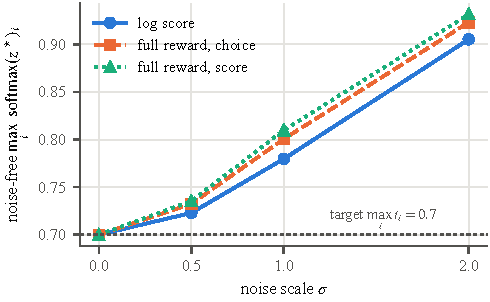
\includegraphics[width=\columnwidth]{figures/fig_e1_toy_bias.pdf}
\caption{E1: noise-free confidence at the optimum of the smoothed objective
for $t=(0.7,0.2,0.1)$. Every reward sharpens beyond the target as $\sigma$
grows.}
\label{fig:e1}
\end{figure}

\subsection{E2: Loss ablation on real data}
\label{sec:e2}

\textbf{Setup.} We replicate Laya's typed-decisions fine-tune on one
A100: initialization from \texttt{convaiinnovations/laya}~\cite{laya_hf},
4 epochs, effective batch 64, AdamW with learning rate $2.5\cdot10^{-5}$ on
the encoder and $10^{-4}$ on the head, cosine decay, clipping at 1.0,
$G{=}4$, $\sigma$ annealed from 0.4 to 0.1, and bf16. We vary only the loss:
CE-only ($w_\mathrm{rl}{=}0$), Laya's RL+CE, RL-only ($w_\mathrm{ce}{=}0$),
and RL+CE at fixed $\sigma\in\{0.5,1,2\}$. We use three seeds for
CE-only, RL+CE and $\sigma{=}1$, and one seed otherwise. All runs share a
fixed budget and are evaluated on their final weights. Temperature is
fitted per (type, option-count bucket) on a held-out 10\% of the
\emph{training} cases. Test: 400 cases, 2000 questions. Our RL+CE
replica reaches accuracy $0.773\pm0.002$ and Brier $0.054\pm0.001$,
against 0.766 and 0.062 in Laya's README.

\textbf{A benchmark caveat.} The gold label of each question equals
$\argmax_i t_i$ on 98.4\% of test rows. It is the teacher's mode, not an
outcome drawn from $t$. Scored as a predictor, the teacher \emph{itself}
has hard-label ECE 0.326 (mean confidence 0.659, accuracy 0.984). A model
that reproduced $t$ perfectly would thus look badly calibrated, and
over-sharpening \emph{reduces} hard-label ECE by moving confidence toward
accuracy. We therefore measure the bias against the target distribution,
using a target-referenced ECE that replaces the 0/1 hit in \eqref{eq:ece}
with the target's probability of the chosen option:
\begin{equation}
\mathrm{ECE}_t=\sum_{b}\frac{|S_b|}{n}\Bigl|\,\overline{c}_{S_b}-\overline{t[\argmax p]}_{S_b}\Bigr|,
\label{eq:softece}
\end{equation}
which is 0 for $p=t$. We also report the sharpness gap
$\overline{\max p}-\overline{\max t}$, NLL and Brier against $t$, fitted
$T$, and, as the plan requires, raw and post-temperature hard-label ECE.
Fig.~\ref{fig:rel} shows the two references side by side.

\begin{figure}[t]
\centering
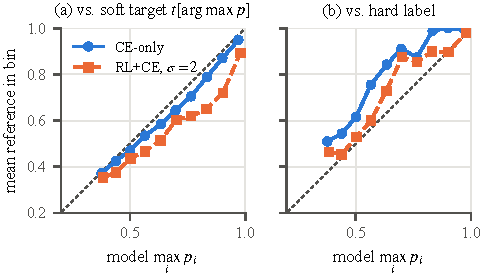
\includegraphics[width=\columnwidth]{figures/fig_reliability.pdf}
\caption{Reliability curves (bins with $\ge$20 rows) for CE-only and RL+CE
at $\sigma{=}2$. (a)~Against the soft target, the $\sigma{=}2$ model is
above the target everywhere (over-sharp). (b)~Against hard labels, every
model appears under-confident, because the labels are the teacher's mode.}
\label{fig:rel}
\end{figure}

\begin{table*}[t]
\caption{E2 on the typed-decisions test set (mean $\pm$ std over seeds; $n$ = seeds). Target-referenced columns first; hard-label columns last.}
\label{tab:e2}
\centering
\footnotesize
\setlength{\tabcolsep}{3pt}
\resizebox{\textwidth}{!}{%
\begin{tabular}{@{}lc cccc c ccc cc c@{}}
\toprule
 & & \multicolumn{4}{c}{vs.\ soft target $t$ (raw)} & post-$T$ & \multicolumn{3}{c}{fitted $T$} & \multicolumn{2}{c}{hard-label ECE} & \\
\cmidrule(lr){3-6}\cmidrule(lr){8-10}\cmidrule(lr){11-12}
Configuration & $n$ & $\overline{\max p}-\overline{\max t}$ & $\mathrm{ECE}_t$ & NLL & Brier & NLL & choice & score & noul & raw & post-$T$ & Acc. \\
\midrule
CE-only ($w_\mathrm{rl}{=}0$) & 3 & $-$0.016{\scriptsize$\pm$0.004} & 0.034{\scriptsize$\pm$0.002} & 0.861{\scriptsize$\pm$0.001} & 0.052{\scriptsize$\pm$0.001} & 0.857{\scriptsize$\pm$0.001} & 1.12{\scriptsize$\pm$0.04} & 1.08{\scriptsize$\pm$0.01} & 1.10{\scriptsize$\pm$0.03} & 0.139{\scriptsize$\pm$0.001} & 0.158{\scriptsize$\pm$0.004} & 0.782{\scriptsize$\pm$0.004} \\
RL+CE, Laya ($\sigma$ 0.4$\to$0.1) & 3 & $-$0.017{\scriptsize$\pm$0.004} & 0.036{\scriptsize$\pm$0.002} & 0.866{\scriptsize$\pm$0.002} & 0.054{\scriptsize$\pm$0.001} & 0.863{\scriptsize$\pm$0.002} & 1.09{\scriptsize$\pm$0.02} & 1.06{\scriptsize$\pm$0.04} & 1.10{\scriptsize$\pm$0.01} & 0.132{\scriptsize$\pm$0.003} & 0.146{\scriptsize$\pm$0.005} & 0.773{\scriptsize$\pm$0.002} \\
RL-only ($w_\mathrm{ce}{=}0$) & 1 & $-$0.024 & 0.032 & 0.868 & 0.055 & 0.866 & 1.07 & 1.06 & 1.15 & 0.127 & 0.141 & 0.760 \\
\midrule
RL+CE, $\sigma{=}0.5$ & 1 & $+$0.001 & 0.054 & 0.870 & 0.057 & 0.862 & 1.15 & 1.12 & 1.22 & 0.114 & 0.144 & 0.774 \\
RL+CE, $\sigma{=}1$ & 3 & $+$0.025{\scriptsize$\pm$0.006} & 0.080{\scriptsize$\pm$0.005} & 0.890{\scriptsize$\pm$0.003} & 0.065{\scriptsize$\pm$0.001} & 0.866{\scriptsize$\pm$0.003} & 1.28{\scriptsize$\pm$0.03} & 1.29{\scriptsize$\pm$0.02} & 1.38{\scriptsize$\pm$0.05} & 0.083{\scriptsize$\pm$0.004} & 0.137{\scriptsize$\pm$0.003} & 0.764{\scriptsize$\pm$0.005} \\
RL+CE, $\sigma{=}2$ & 1 & $+$0.060 & 0.111 & 0.932 & 0.075 & 0.865 & 1.49 & 1.57 & 1.72 & 0.056 & 0.145 & 0.774 \\
\midrule
\textit{Teacher $t$ as predictor} & -- & $0$ & $0$ & -- & $0$ & -- & -- & -- & -- & 0.326 & -- & 0.984 \\
\bottomrule

\end{tabular}}
\end{table*}

\begin{figure}[t]
\centering
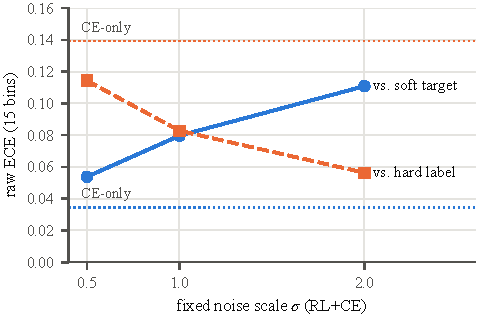
\includegraphics[width=\columnwidth]{figures/fig_ece_crossing.pdf}
\caption{As fixed $\sigma$ grows, target-referenced ECE rises while
hard-label ECE falls: the same models ranked in opposite order. Dotted lines
show CE-only.}
\label{fig:ece}
\end{figure}

\begin{figure}[t]
\centering
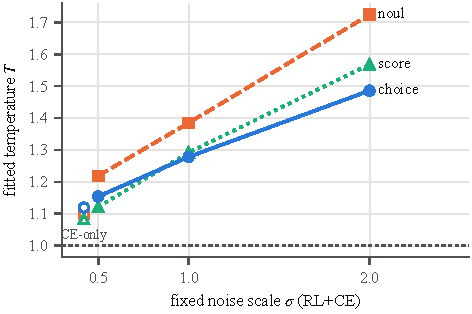
\includegraphics[width=\columnwidth]{figures/fig_temperature.pdf}
\caption{Fitted temperature per question type versus fixed $\sigma$
(RL+CE); hollow markers show CE-only. $T>1$ means the raw outputs are
sharper than the targets.}
\label{fig:temp}
\end{figure}

\textbf{The bias appears at full scale.} Table~\ref{tab:e2} and
Figs.~\ref{fig:ece}--\ref{fig:temp} show that at fixed $\sigma$ every
target-referenced measure worsens monotonically. The sharpness gap goes
from $+0.001$ to $+0.025$ to $+0.060$ and $\mathrm{ECE}_t$ from 0.054 to
0.080 to 0.111, reaching 3.3$\times$ CE-only. Fitted $T$ rises for every
type (noul: 1.22, 1.38, 1.72) and NLL rises from 0.870 to 0.932. The
three-seed spread at $\sigma{=}1$ is an order of magnitude smaller than
these steps. Hard-label ECE falls over the same runs (0.114, 0.083,
0.056), as the caveat predicts. Temperature scaling recovers most of the
NLL loss (0.932 to 0.865 at $\sigma{=}2$), consistent with a systematic
sharpening rather than degraded ranking; accuracy is unchanged within
noise.

\textbf{At Laya's own schedule the RL term does nothing useful.} RL+CE and
CE-only are indistinguishable in sharpness ($-0.017$ vs $-0.016$),
$\mathrm{ECE}_t$ (0.036 vs 0.034) and fitted $T$. CE-only is better on NLL
for every seed (0.861 vs 0.866, including after temperature scaling), on
Brier (0.052 vs 0.054) and on accuracy (0.782 vs 0.773). RL-only (one seed)
is the least accurate (0.760) but is not over-sharp. This matches the
$O(\sigma^2)$ remark: with $\sigma\le0.4$ the bias is too small to show,
and what remains is estimator noise. The raw hard-label ECE favors RL+CE
(0.132 vs 0.139) only because of the caveat above.

\textbf{Where the sharpening lands.} Split by target-entropy tercile
(Table~\ref{tab:entropy}), every model, CE-only included, is under-sharp
on peaked targets and over-sharp on flat ones, a regression toward typical
confidence. Increasing $\sigma$ adds a near-uniform upward shift across
terciles. The mean gap of CE-only near zero therefore reflects two
opposite biases, not the absence of bias.

\begin{table}[t]
\caption{Sharpness gap $\overline{\max p}-\overline{\max t}$ by target-entropy tercile (mean $H(t)$: 0.38 / 0.82 / 1.12 nats).}
\label{tab:entropy}
\centering
\footnotesize
\begin{tabular}{@{}lccc@{}}
\toprule
Configuration & peaked & mid & flat \\
\midrule
CE-only ($w_\mathrm{rl}{=}0$) & $-$0.056 & $-$0.017 & $+$0.026 \\
RL+CE, Laya ($\sigma$ 0.4$\to$0.1) & $-$0.059 & $-$0.017 & $+$0.025 \\
RL-only ($w_\mathrm{ce}{=}0$) & $-$0.067 & $-$0.024 & $+$0.019 \\
RL+CE, $\sigma{=}0.5$ & $-$0.046 & $+$0.002 & $+$0.047 \\
RL+CE, $\sigma{=}1$ & $-$0.028 & $+$0.026 & $+$0.076 \\
RL+CE, $\sigma{=}2$ & $+$0.008 & $+$0.069 & $+$0.104 \\
\bottomrule

\end{tabular}
\end{table}

\subsection{E3: Gradient quality}
\label{sec:e3}

Every 10 optimizer steps we compare \eqref{eq:es} with the CE gradient,
both taken with respect to the logits and each from a fresh noise draw
(Table~\ref{tab:e3}, Fig.~\ref{fig:grad}). Under Laya's schedule the RL
gradient is 8$\times$ the CE gradient at $\sigma{=}0.4$ and 87$\times$ at
$\sigma{=}0.1$. Before clipping it therefore dominates the update, and its
alignment with CE is only moderate (cosine $\approx0.65$). In the fixed-$\sigma$
runs, where $\sigma$ is not confounded with training progress, the norm
ratio scales as $1/\sigma$ (ratio$\times\sigma\approx$ 5.2, 4.9, 4.3) and
the alignment falls from 0.60 to 0.52 to 0.37 as the smoothed gradient
departs from the CE gradient. Despite its size, the RL term leaves the
final model essentially where CE alone would put it. This is consistent
with a noisy, roughly unbiased proxy for the CE direction at small
$\sigma$.

\begin{table}[t]
\caption{E3: RL vs.\ CE logit gradients ($n$ = runs).}
\label{tab:e3}
\centering
\footnotesize
\begin{tabular}{@{}lccc@{}}
\toprule
$\sigma$ & $n$ & $\cos(\nabla L_\mathrm{RL},\nabla L_\mathrm{CE})$ & $\|\nabla L_\mathrm{RL}\|/\|\nabla L_\mathrm{CE}\|$ \\
\midrule
0.4 (annealed) & 8 & 0.66{\scriptsize$\pm$0.04} & 8.4{\scriptsize$\pm$0.8} \\
0.3 (annealed) & 8 & 0.64{\scriptsize$\pm$0.04} & 16.9{\scriptsize$\pm$3.4} \\
0.2 (annealed) & 8 & 0.66{\scriptsize$\pm$0.04} & 34.0{\scriptsize$\pm$5.3} \\
0.1 (annealed) & 8 & 0.65{\scriptsize$\pm$0.04} & 86.6{\scriptsize$\pm$17.0} \\
\midrule
0.5 (fixed) & 1 & 0.60 & 10.4 \\
1.0 (fixed) & 3 & 0.52{\scriptsize$\pm$0.02} & 4.9{\scriptsize$\pm$0.5} \\
2.0 (fixed) & 1 & 0.37 & 2.2 \\
\bottomrule

\end{tabular}
\end{table}

\begin{figure}[t]
\centering
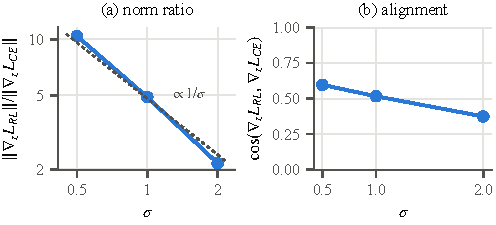
\includegraphics[width=\columnwidth]{figures/fig_gradients.pdf}
\caption{E3 at fixed $\sigma$: (a)~the RL/CE gradient-norm ratio follows
$1/\sigma$; (b)~alignment with the CE gradient falls as $\sigma$ grows.}
\label{fig:grad}
\end{figure}

\subsection{Reproducibility}
A second run of RL+CE seed 42 reproduced the first closely (NLL 0.864 /
0.867, accuracy 0.772 / 0.772), though not bitwise. One earlier seed-42
run, the first job on a fresh machine, matched the others at step 1 and
then diverged to accuracy 0.697 and NLL 0.936. Its cause is undetermined
(a first-time kernel compilation is the leading suspect). It is excluded
from the tables and archived with the results.

% =====================================================================
\section{Toward a Principled RLCD Pipeline}
\label{sec:principled}

If the goal is calibrated typed distributions, the analysis above implies
the following. Stage one is distillation, i.e.\ soft CE against targets
from a controlled data engine: exact labels where the latent state is
known, known posteriors where noise is injected, and teacher ensembles
otherwise. Reinforcement learning should be reserved for what CE cannot
provide: non-differentiable workflow rewards, sequential decisions
(temporal-difference targets), and a separate action/escalation head whose
utility never feeds the probability head. Calibration should then be
enforced where it is measurable: mining (type, $K$, length, language)
buckets with high target-referenced error for more data, consistency
regularizers (negation pairs summing to one, option-permutation and
irrelevant-context invariance), and temperature per (type, $K$). A large
fitted temperature signals that an upstream stage distorted the
distributions. Evaluation should report raw target-referenced calibration
next to post-temperature numbers, and use labels drawn from distributions
(e.g.\ multi-annotator sets such as ChaosNLI~\cite{nie2020chaosnli})
whenever outcome calibration is claimed. This is a proposal, not a
description of any existing system.

% =====================================================================
\section{Limitations}

Jev is closed: Sec.~\ref{sec:jev} is inference from public claims, and
nothing here tests Jev. We use one benchmark, whose labels are teacher
modes; the benchmark's ceiling of teacher self-agreement (0.735) makes
small accuracy gaps weak evidence, so we lead with proper scores and fitted
temperatures. Three configurations have a single seed. All runs start from
a checkpoint that Laya had already trained with RLCD, which favors
RL-only. Proposition~\ref{prop:binary} covers the log score with $K{=}2$;
the general-$K$ and full-reward cases rest on numerics. The E3 diagnostics
are logit-level, not parameter-level. The model scale is fixed
(421M parameters).

% =====================================================================
\section{Conclusion}

Laya's RL term optimizes a noise-smoothed proper score. As $\sigma\to0$
that objective becomes the CE the model already minimizes, and for
$\sigma>0$ its optimum is over-sharp at inference. We prove this for
binary questions, show it numerically for Laya's full reward, and observe
it at full scale: fitted temperature and target-referenced calibration
error grow monotonically with $\sigma$. At Laya's own small, annealed
$\sigma$, the RL term dominates the gradient yet leaves calibration
unchanged and proper scores slightly worse than CE-only. On this evidence,
the calibration of Laya-style typed-decision models comes from distillation
and temperature scaling, not from the RL term. On benchmarks whose labels
are teacher modes, hard-label ECE should not be used to argue otherwise.

\section*{Acknowledgment}
The author thanks the Laya authors for releasing their code, checkpoints,
notebook and a candid README, without which this analysis would not have
been possible.

\bibliographystyle{IEEEtran}
\bibliography{refs}

% =====================================================================
\appendices

\section{Reproduction details}
\label{app:repro}

\textbf{Weight parity.} Laya's \texttt{model.safetensors} contains 206
tensors. Of these, 201 map one-to-one onto our model (encoder, head, type
embedding, scorer). The five others are the unused action head and a
per-type temperature. Tokenizers are identical to ModernBERT-large's.
Before fine-tuning, the released base checkpoint already has hard-label
ECE 0.215 on a 60-row slice. Its shipped per-type temperatures
(1.64 / 1.25 / 1.98) are all $>1$.

\textbf{Deliberate differences from the notebook.} bf16 instead of
fp16 with loss scaling; a case-level instead of row-level calibration
split; temperature per (type, $K$-bucket) instead of per type; one GPU
with effective batch 64 instead of two GPUs.

\textbf{Compute.} One A100-SXM4-40GB. Each run took about 8 minutes
(5.5 of training); the 13 runs plus setup cost about 2.4 GPU-hours.

\begin{table}[h]
\caption{All E2 runs (test set; raw logits).}
\label{tab:allruns}
\centering
\scriptsize
\setlength{\tabcolsep}{2.4pt}
\resizebox{\columnwidth}{!}{%
\begin{tabular}{@{}lccccccccc@{}}
\toprule
Run & gap & $\mathrm{ECE}_t$ & NLL & Brier & $T_c$ & $T_s$ & $T_n$ & ECE & Acc. \\
\midrule
ce\_only\_seed42 & $-$0.013 & 0.035 & 0.860 & 0.051 & 1.10 & 1.09 & 1.13 & 0.140 & 0.785 \\
ce\_only\_seed43 & $-$0.020 & 0.032 & 0.862 & 0.052 & 1.09 & 1.07 & 1.07 & 0.139 & 0.778 \\
ce\_only\_seed44 & $-$0.014 & 0.036 & 0.862 & 0.051 & 1.17 & 1.09 & 1.09 & 0.138 & 0.783 \\
laya\_rlce\_seed42 & $-$0.016 & 0.038 & 0.864 & 0.053 & 1.10 & 1.01 & 1.11 & 0.129 & 0.772 \\
laya\_rlce\_seed42\_rep2 & $-$0.018 & 0.035 & 0.867 & 0.055 & 1.06 & 1.08 & 1.10 & 0.131 & 0.772 \\
laya\_rlce\_seed43 & $-$0.014 & 0.037 & 0.867 & 0.054 & 1.06 & 1.09 & 1.09 & 0.131 & 0.775 \\
laya\_rlce\_seed44 & $-$0.021 & 0.034 & 0.867 & 0.055 & 1.11 & 1.06 & 1.10 & 0.135 & 0.772 \\
rl\_only\_seed42 & $-$0.024 & 0.032 & 0.868 & 0.055 & 1.07 & 1.06 & 1.15 & 0.127 & 0.760 \\
rlce\_sigma0p5\_fixed\_seed42 & $+$0.001 & 0.054 & 0.870 & 0.057 & 1.15 & 1.12 & 1.22 & 0.114 & 0.774 \\
rlce\_sigma1\_fixed\_seed42 & $+$0.030 & 0.084 & 0.888 & 0.064 & 1.26 & 1.28 & 1.37 & 0.081 & 0.770 \\
rlce\_sigma1\_fixed\_seed43 & $+$0.019 & 0.074 & 0.893 & 0.067 & 1.26 & 1.29 & 1.44 & 0.088 & 0.761 \\
rlce\_sigma1\_fixed\_seed44 & $+$0.025 & 0.081 & 0.889 & 0.065 & 1.31 & 1.31 & 1.34 & 0.080 & 0.762 \\
rlce\_sigma2\_fixed\_seed42 & $+$0.060 & 0.111 & 0.932 & 0.075 & 1.49 & 1.57 & 1.72 & 0.056 & 0.774 \\
\bottomrule

\end{tabular}}
\end{table}

\section{The RLCD loss (condensed from our port)}
\begin{lstlisting}[language=Python]
k   = mask.sum(-1, keepdim=True).clamp(min=2)
eps = torch.randn((G,) + z.shape) * sigma * mask
eps = (eps - eps.sum(-1, keepdim=True) / k) * mask
zs  = z.detach().unsqueeze(0) + eps
q   = torch.softmax(zs.masked_fill(~mask, -1e4), -1)
with torch.no_grad():
    r   = proper_reward(q, t, qtype, mask, w_sph=0.75)
    adv = r - r.mean(0, keepdim=True)
    adv = adv / (adv.std() + 1e-6)
logp    = -(((zs - z) ** 2) * mask).sum(-1) / (2 * sigma**2)
loss_rl = -(adv * logp).mean()
loss_ce = -(t * torch.log_softmax(z, -1)).sum(-1).mean()
loss    = w_rl * loss_rl + w_ce * loss_ce
\end{lstlisting}

\end{document}
